\documentclass[preview]{standalone}
\usepackage{graphicx}
\usepackage{subcaption}

\begin{document}
\begin{figure}
\captionsetup[subfigure]{justification=centering}
  \begin{subfigure}[b]{.49\columnwidth}
    \centering
    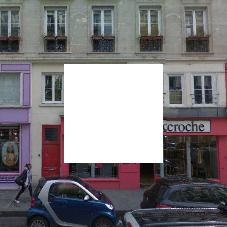
\includegraphics[width=0.99\linewidth,height=0.99\linewidth]{figures/chapter02/0_data_ctx_overlap}
    \caption{Input context}
  \end{subfigure}
  \begin{subfigure}[b]{.49\columnwidth}
    \centering
    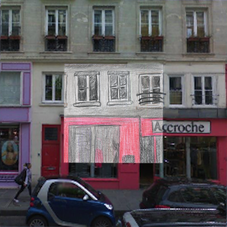
\includegraphics[width=0.99\linewidth,height=0.99\linewidth]{figures/chapter02/artist_overlap_227}
    \caption{Human artist}
  \end{subfigure}
\medskip 
  \begin{subfigure}[b]{.49\columnwidth}
    \centering
    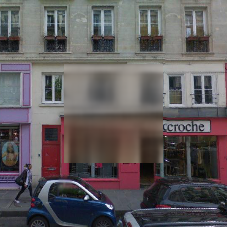
\includegraphics[width=0.99\linewidth,height=0.99\linewidth]{figures/chapter02/0_merge_l2_overlap}
    \caption{Context Encoder\\($L2$ loss)}
  \end{subfigure}
  \begin{subfigure}[b]{.49\columnwidth}
    \centering
    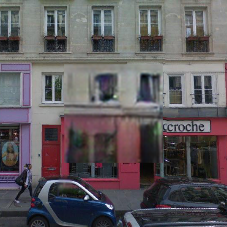
\includegraphics[width=0.99\linewidth,height=0.99\linewidth]{figures/chapter02/paris_m21_full_0017_pred_highres}
    \caption{Context Encoder\\($L2$ + Adversarial loss)}
  \end{subfigure}
\end{figure}
\end{document}